\section{Diagramme de Séquence}\label{sec:diagramme_sequence}

\begin{definition}[Diagramme de séquence]
Un diagramme de séquence (Sequence Diagram) est un type de diagramme UML qui représente la séquence temporelle d’échange de messages entre les objets réalisant une certaine tâche
\end{definition}

Il est utilisé pour modéliser le comportement dynamique d'un système en décrivant les interactions entre objets à un niveau de détail plus fin que le diagramme de cas d'utilisation.




\subsection{Éléments}
La dimension verticale représente le temps.
La syntaxe d'un diagramme de séquence comprend les éléments suivants :
\begin{itemize}
\item Objet : un objet est un élément du système qui possède des comportements et des données. Il est représenté par un rectangle constitué du nom de l'objet soligné et précédé de : . Les objets sont disposés horizontalement.
\item Message : Un message est représenté par une flèche joignant deux boîtes. d’activation. Il a un nom et peut aussi avoir une liste d’arguments et une valeur de retour.
\item Lifeline :  Une ligne de vie (lifeline) est accrochée à chaque objet
\item Activation : La ligne de vie s’épaissie pour devenir une boîte d’activation lorsque l’objet est actif, c.à.d., durant la période d’activation..
\end{itemize}

\begin{figure}[H]
\centering
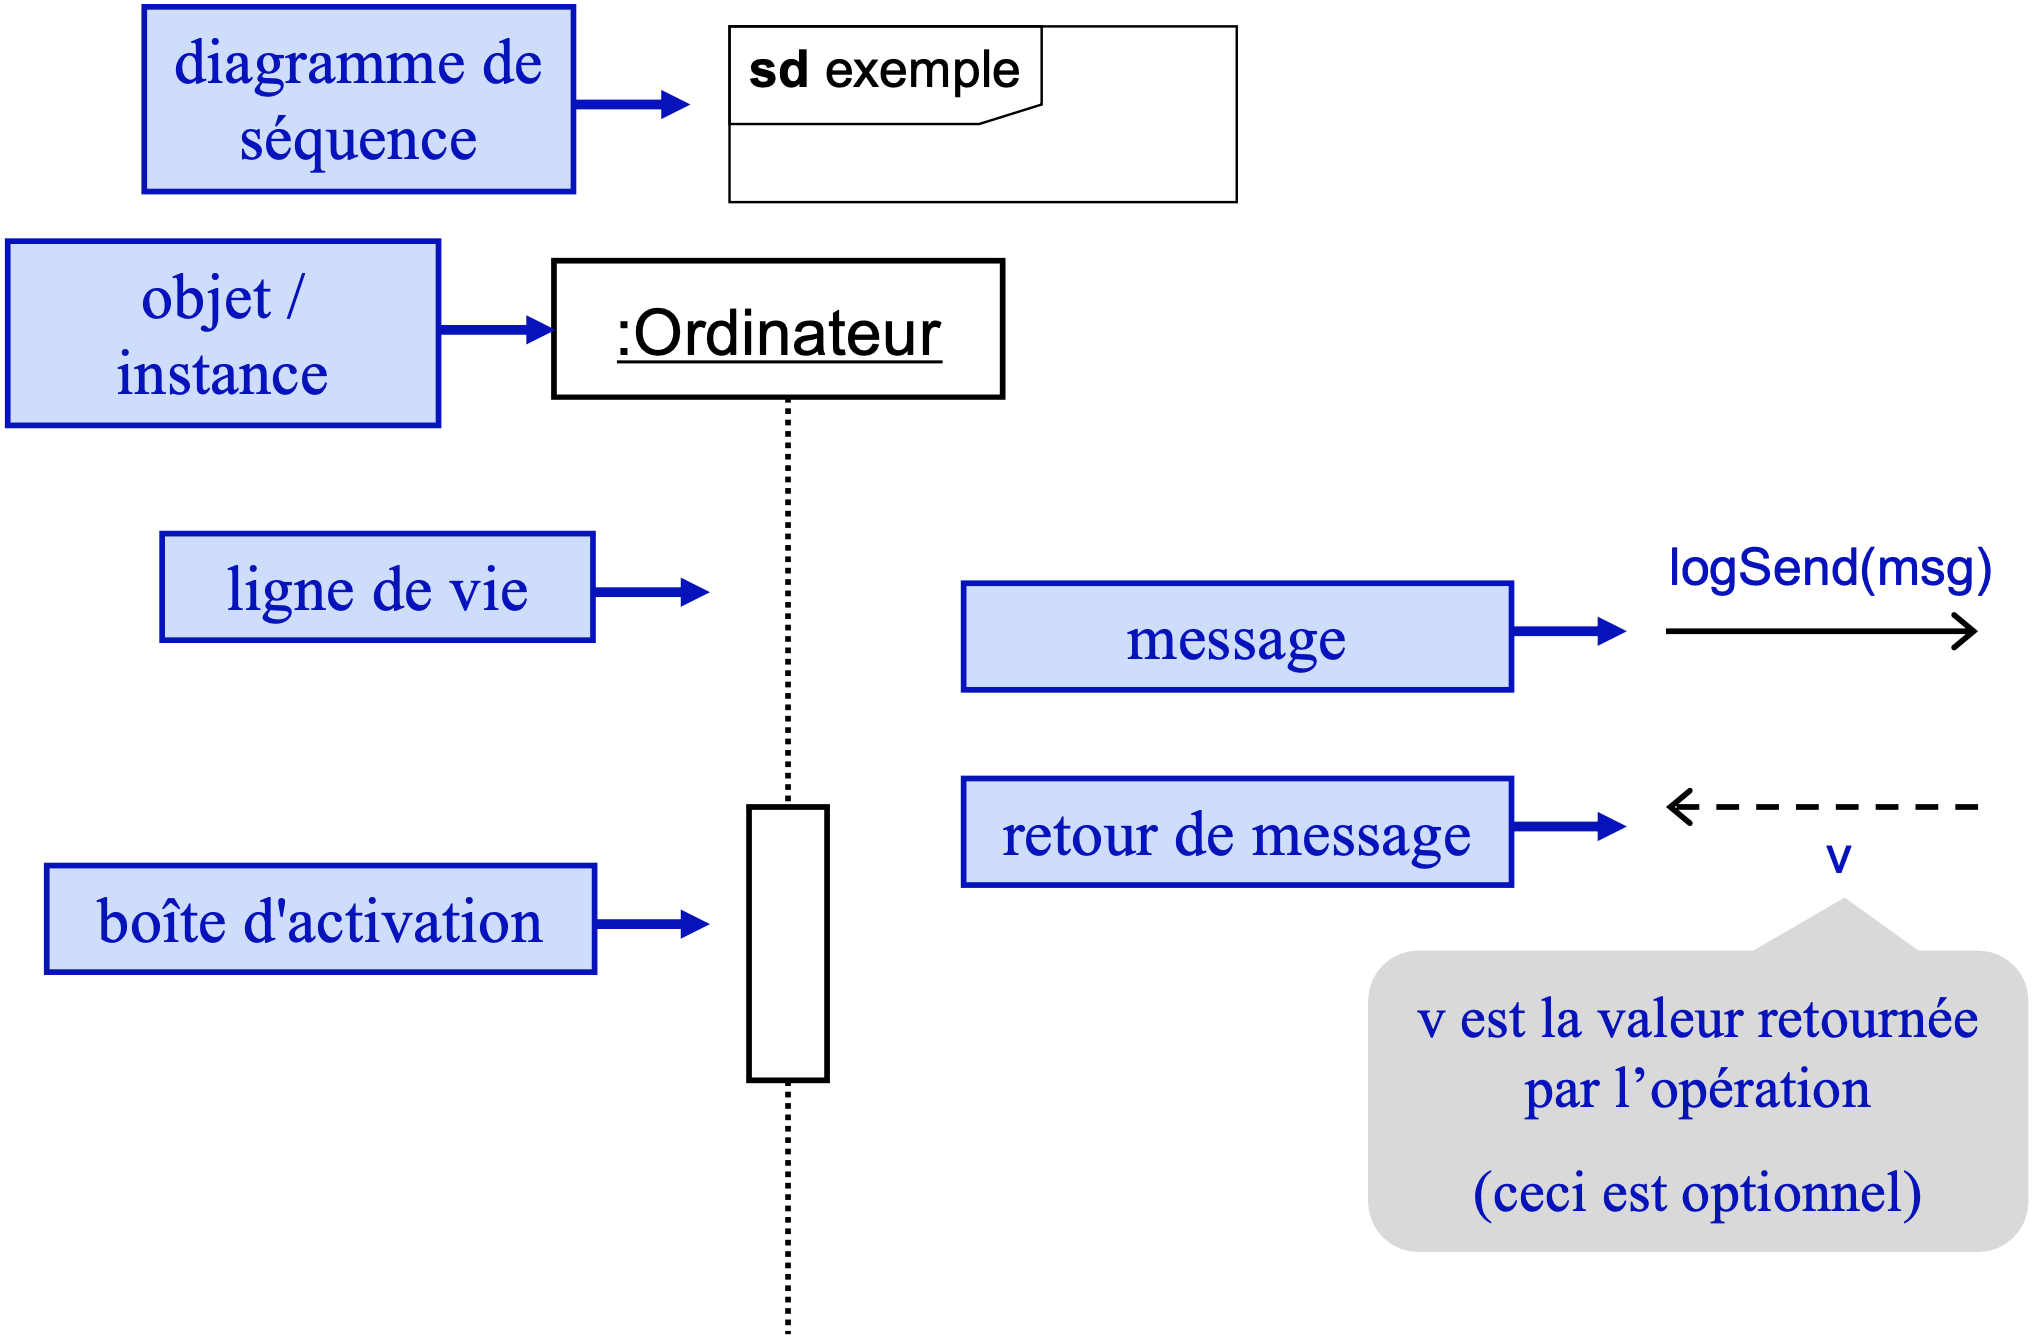
\includegraphics[width=\textwidth]{./Images/Diagrammes/diagram_sequence_elements.png}
\caption{Éléments d'un diagramme de séquence}
\label{fig:diagram_sequence_elements}
\end{figure}


\subsection{Étapes}
Pour construire un diagramme de séquence, vous pouvez suivre ces étapes :
\begin{enumerate}
\item Identifiez les acteurs (personnes ou systèmes) qui participent à la séquence d'interactions que vous voulez modéliser. Chaque acteur sera représenté par un rectangle horizontal dans le diagramme.
\item Définissez les étapes de la séquence d'interactions que vous voulez modéliser. Chaque étape sera représentée par un rectangle vertical dans le diagramme.
\item Déterminez l'ordre dans lequel les étapes de la séquence doivent être exécutées. Utilisez des flèches pour relier les étapes entre elles dans le bon ordre.
\item Ajoutez les détails nécessaires aux étapes, tels que les messages envoyés entre les acteurs et les événements qui déclenchent les étapes suivantes.
\end{enumerate}


\subsection{Fragments Combinés}
\begin{definition}[Fragment Combiné]
Un fragment combiné:
\begin{itemize}
\item représente des articulations d'intéractions
\item permet de décrire des diagrammes de séquence de
manière compacte
\item peut faire intervenir l'ensemble des entités participant
au scénario ou juste un sous-ensemble
\end{itemize}
Il est défini par un opérateur qui détermine sa sémantique et des opérandes.\\
=> Exemples: ref,opt,alt,loop,break,critical,par,neg, \dots
\end{definition}


\begin{table}[H]
\centering
\caption{Opérateurs de boucle et de condition dans les diagrammes de séquence UML}
\label{tbl:uml_loop_cond}
\begin{tabular}{p{7em}|p{18em}|p{14em}}
\toprule
Opérateur & Description & Exemple \\
\midrule
\multirow{2}{*}{loop} 
& Boucle avec contrainte de garde indiquant le nombre de répétitions & loop [min=0, max=5] \\
\cmidrule(lr){2-3}
& Boucle avec contrainte de garde indiquant une condition booléenne à respecter & loop [condition] \\
\cmidrule(lr){1-3}
\multirow{2}{*}{alt} 
& Alternative avec opérande else & alt [condition] then ... else ... \\
\cmidrule(lr){2-3}
& Alternative sans opérande else & alt [condition] then ... \\
\cmidrule(lr){1-3}
opt & Choix optionnel sans opérande else & opt [condition] then ... \\
\cmidrule(lr){1-3}
break & Si condition remplie, ignore le reste des instructions & [condition] then ... \\
\cmidrule(lr){1-3}
ref & Référence à un autre diagramme de séquence & \\
\cmidrule(lr){1-3}
par & Instructions exécutées en parallèle & \\
\cmidrule(lr){1-3}
neg & Si condition remplie, ignore les instructions du fragment & \\
\cmidrule(lr){1-3}
critical & Fragment à exécuté de façon atomique & \\
\bottomrule
\end{tabular}
\end{table}


\begin{figure}[H]
\centering
\begin{subfigure}{0.55\textwidth}
  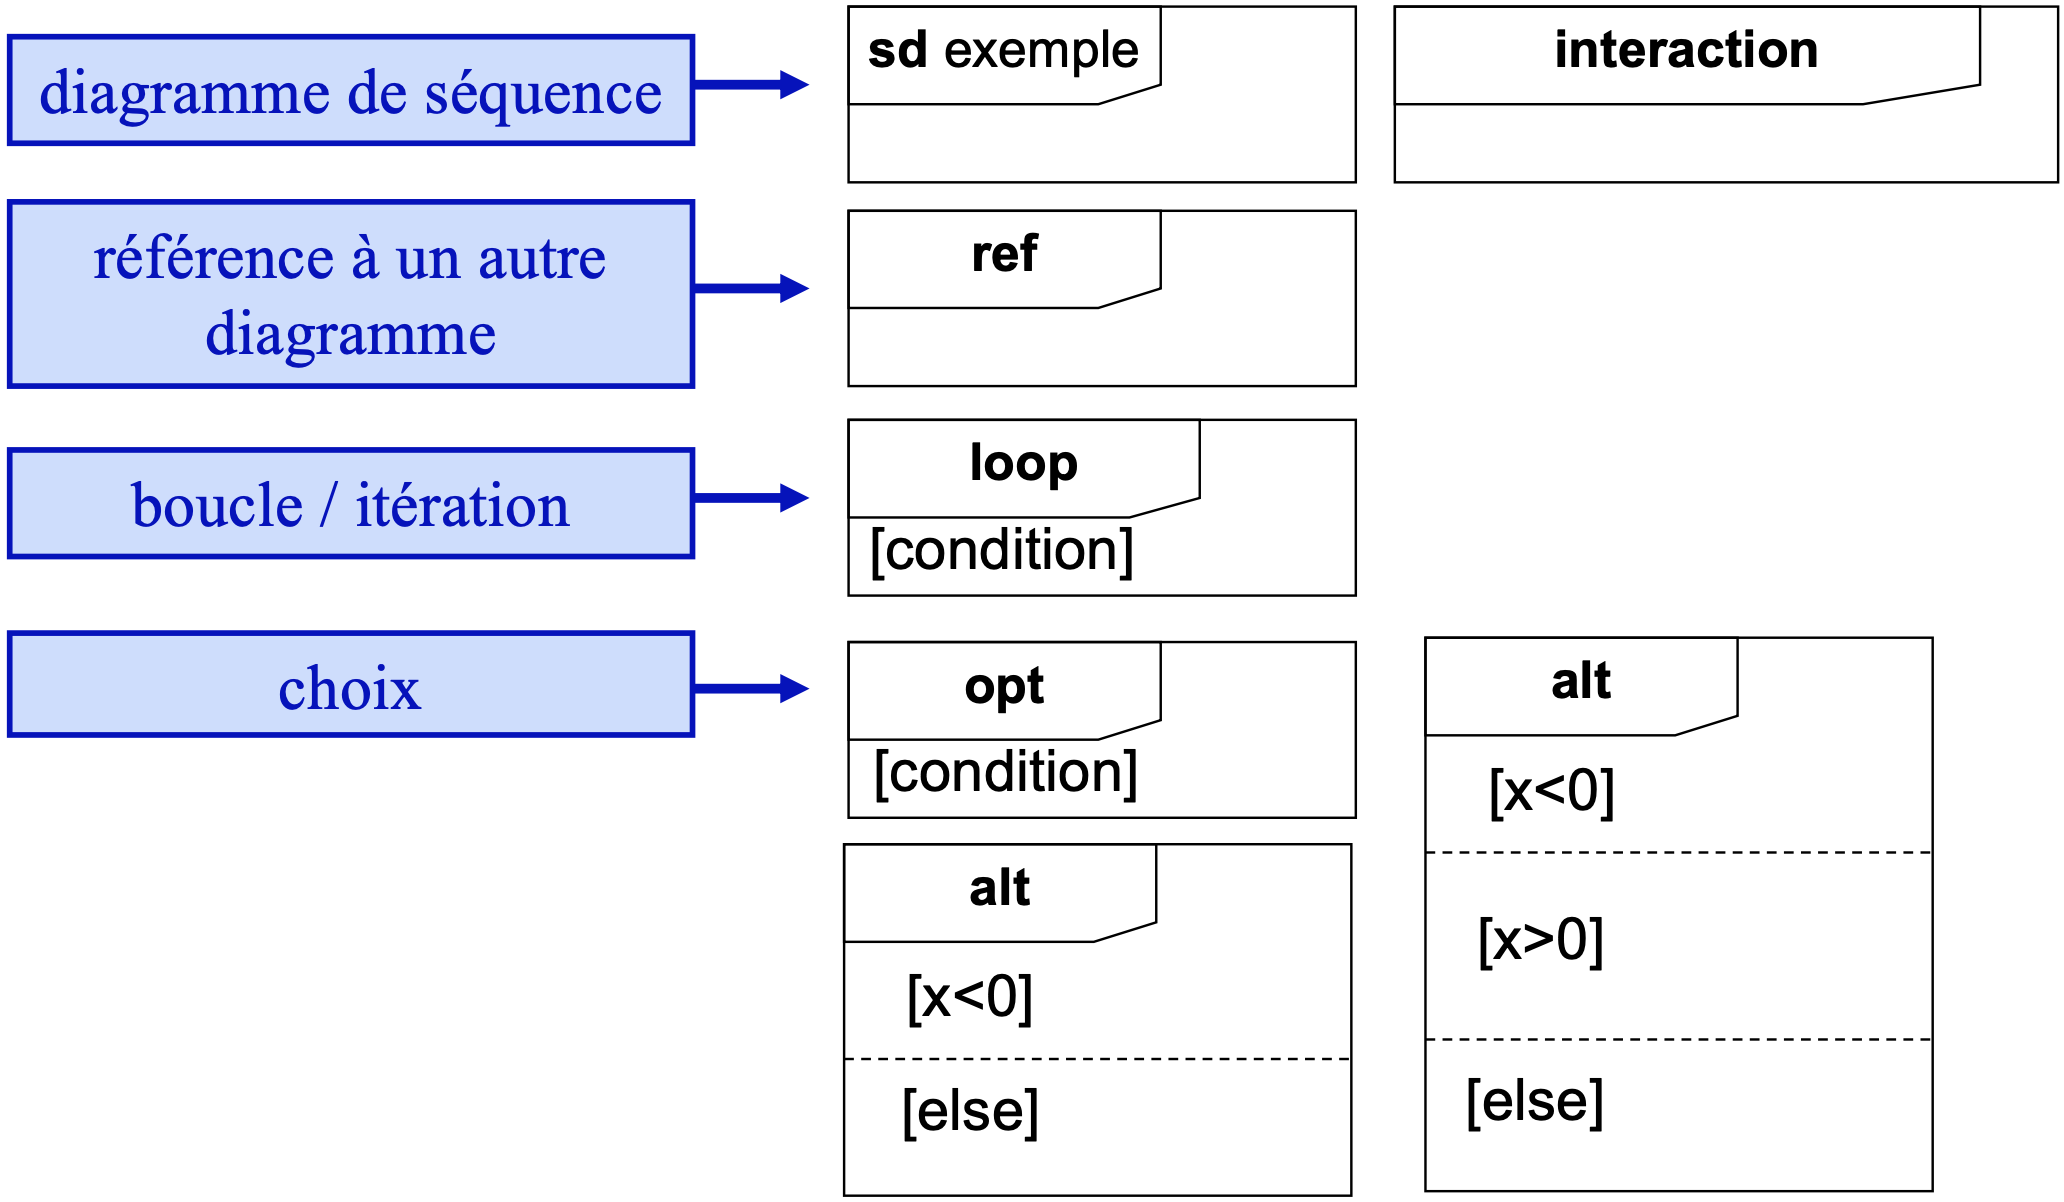
\includegraphics[width=\textwidth]{./Images/Diagrammes/diagram_sequence_fragmentscombines1.png}
  %\caption{}
  \label{fig:diagram_sequence_fc1}
\end{subfigure}
\begin{subfigure}{0.4\textwidth}
  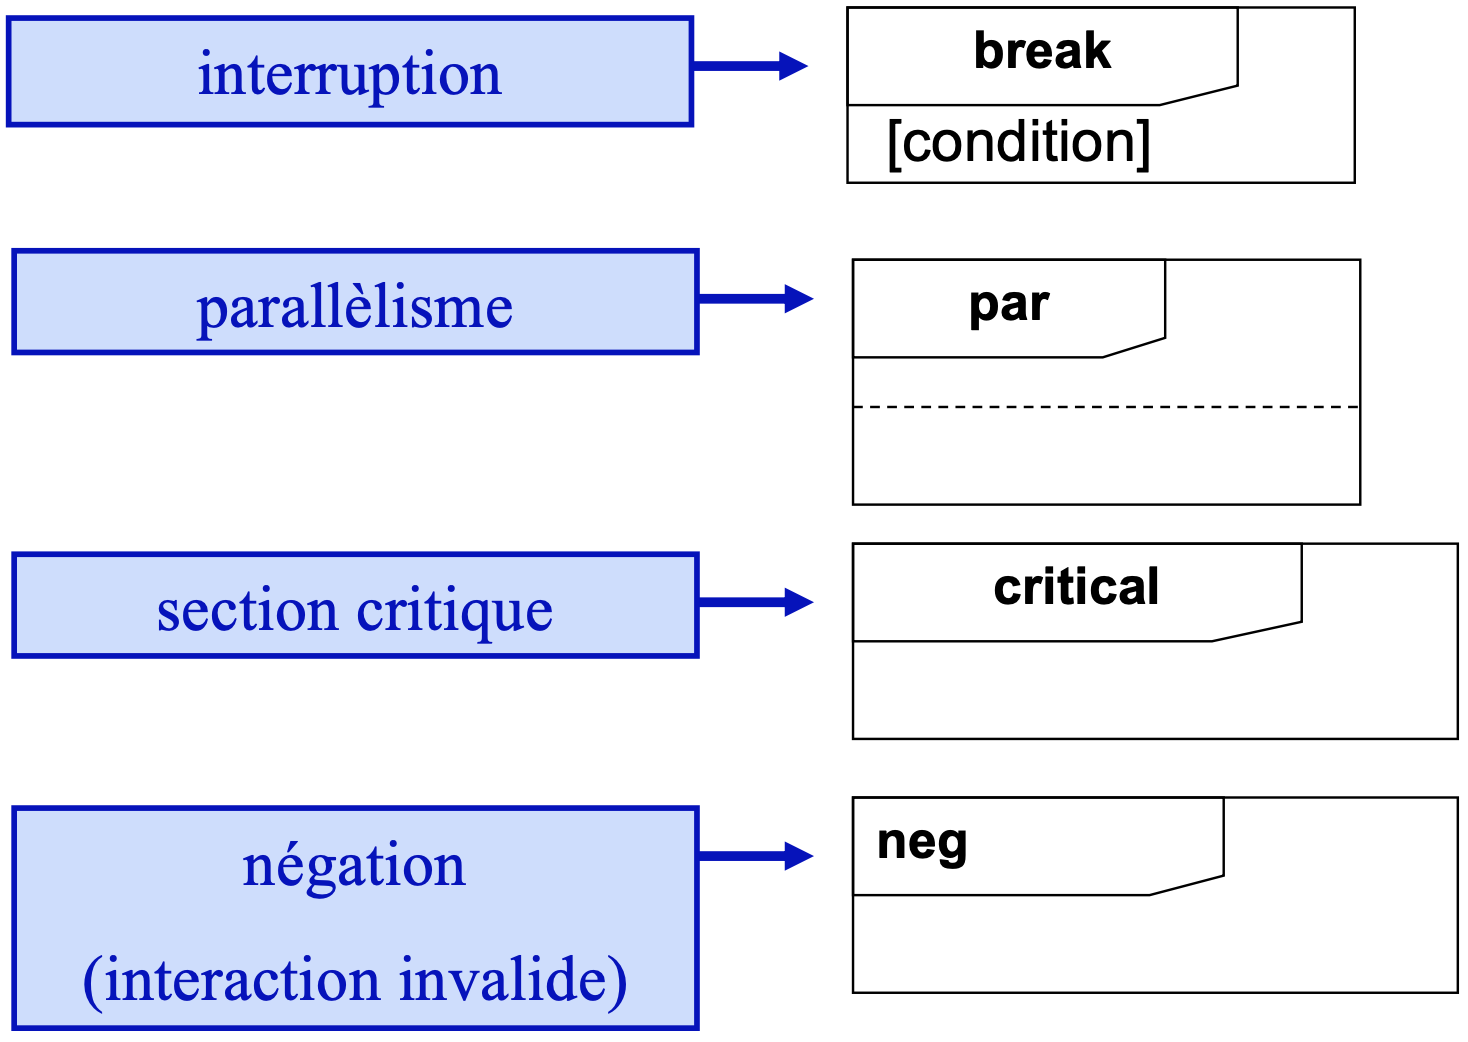
\includegraphics[width=\textwidth]{./Images/Diagrammes/diagram_sequence_fragmentscombines.png}
  %\caption{}
  \label{fig:diagram_sequence_fc2}
\end{subfigure}
\caption{Fragments Combinés}
\end{figure}

\begin{figure}[H]
\centering
\begin{subfigure}{0.45\textwidth}
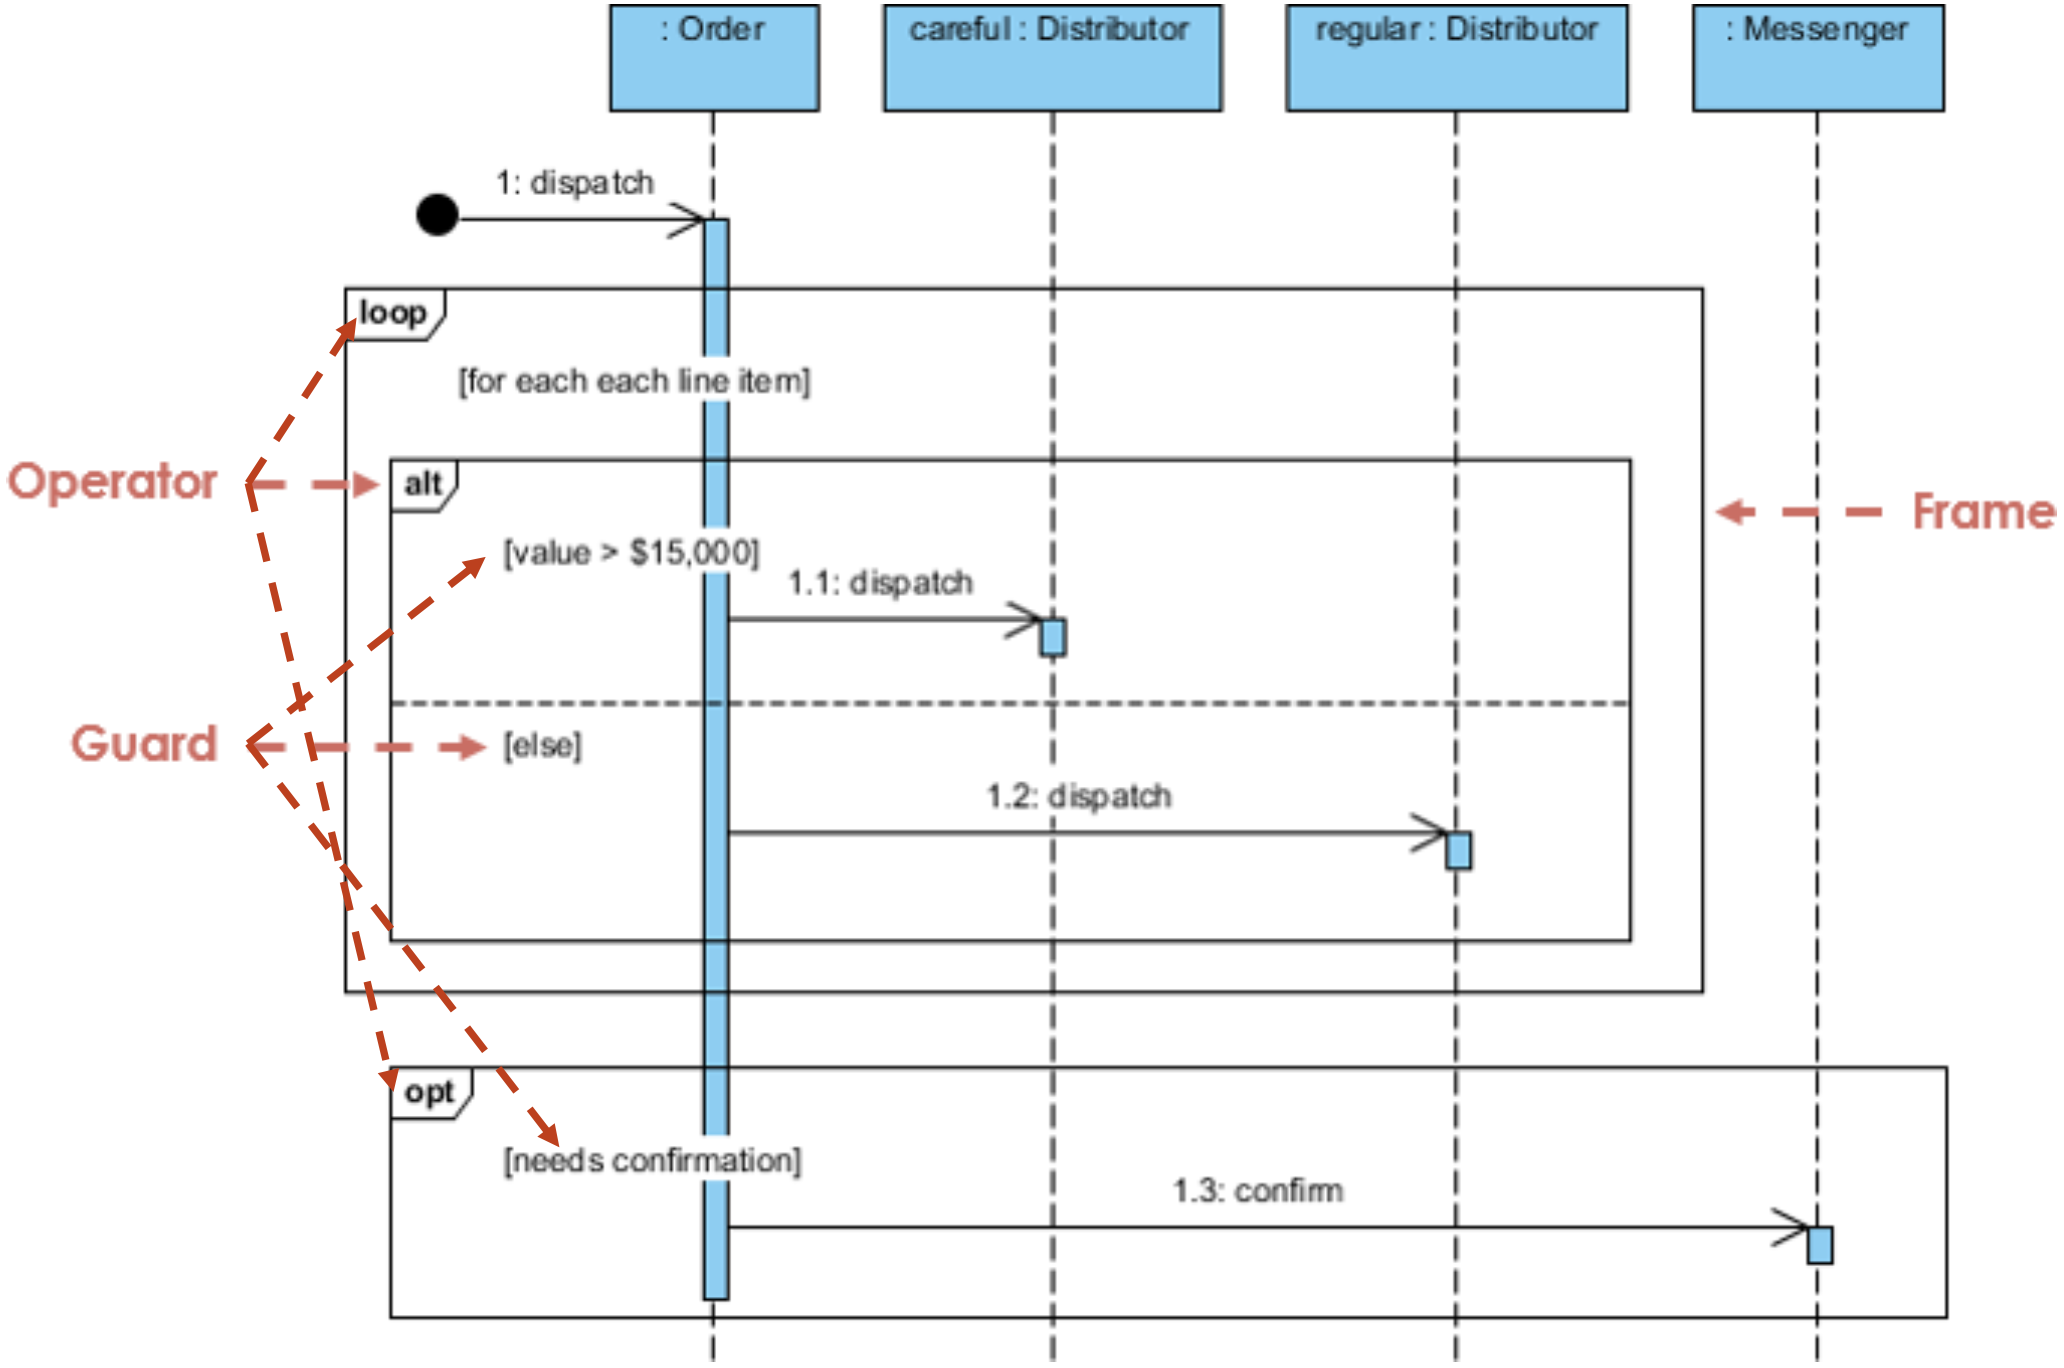
\includegraphics[width=\textwidth]{./Images/Diagrammes/diagram_sequence_ex_fragmentscombines.png}
\caption{Fragments combinés \og Loop Alt Opt\fg}
\label{fig:diagram_sequence_fc_loopaltopt}
\end{subfigure}
\begin{subfigure}{0.45\textwidth}
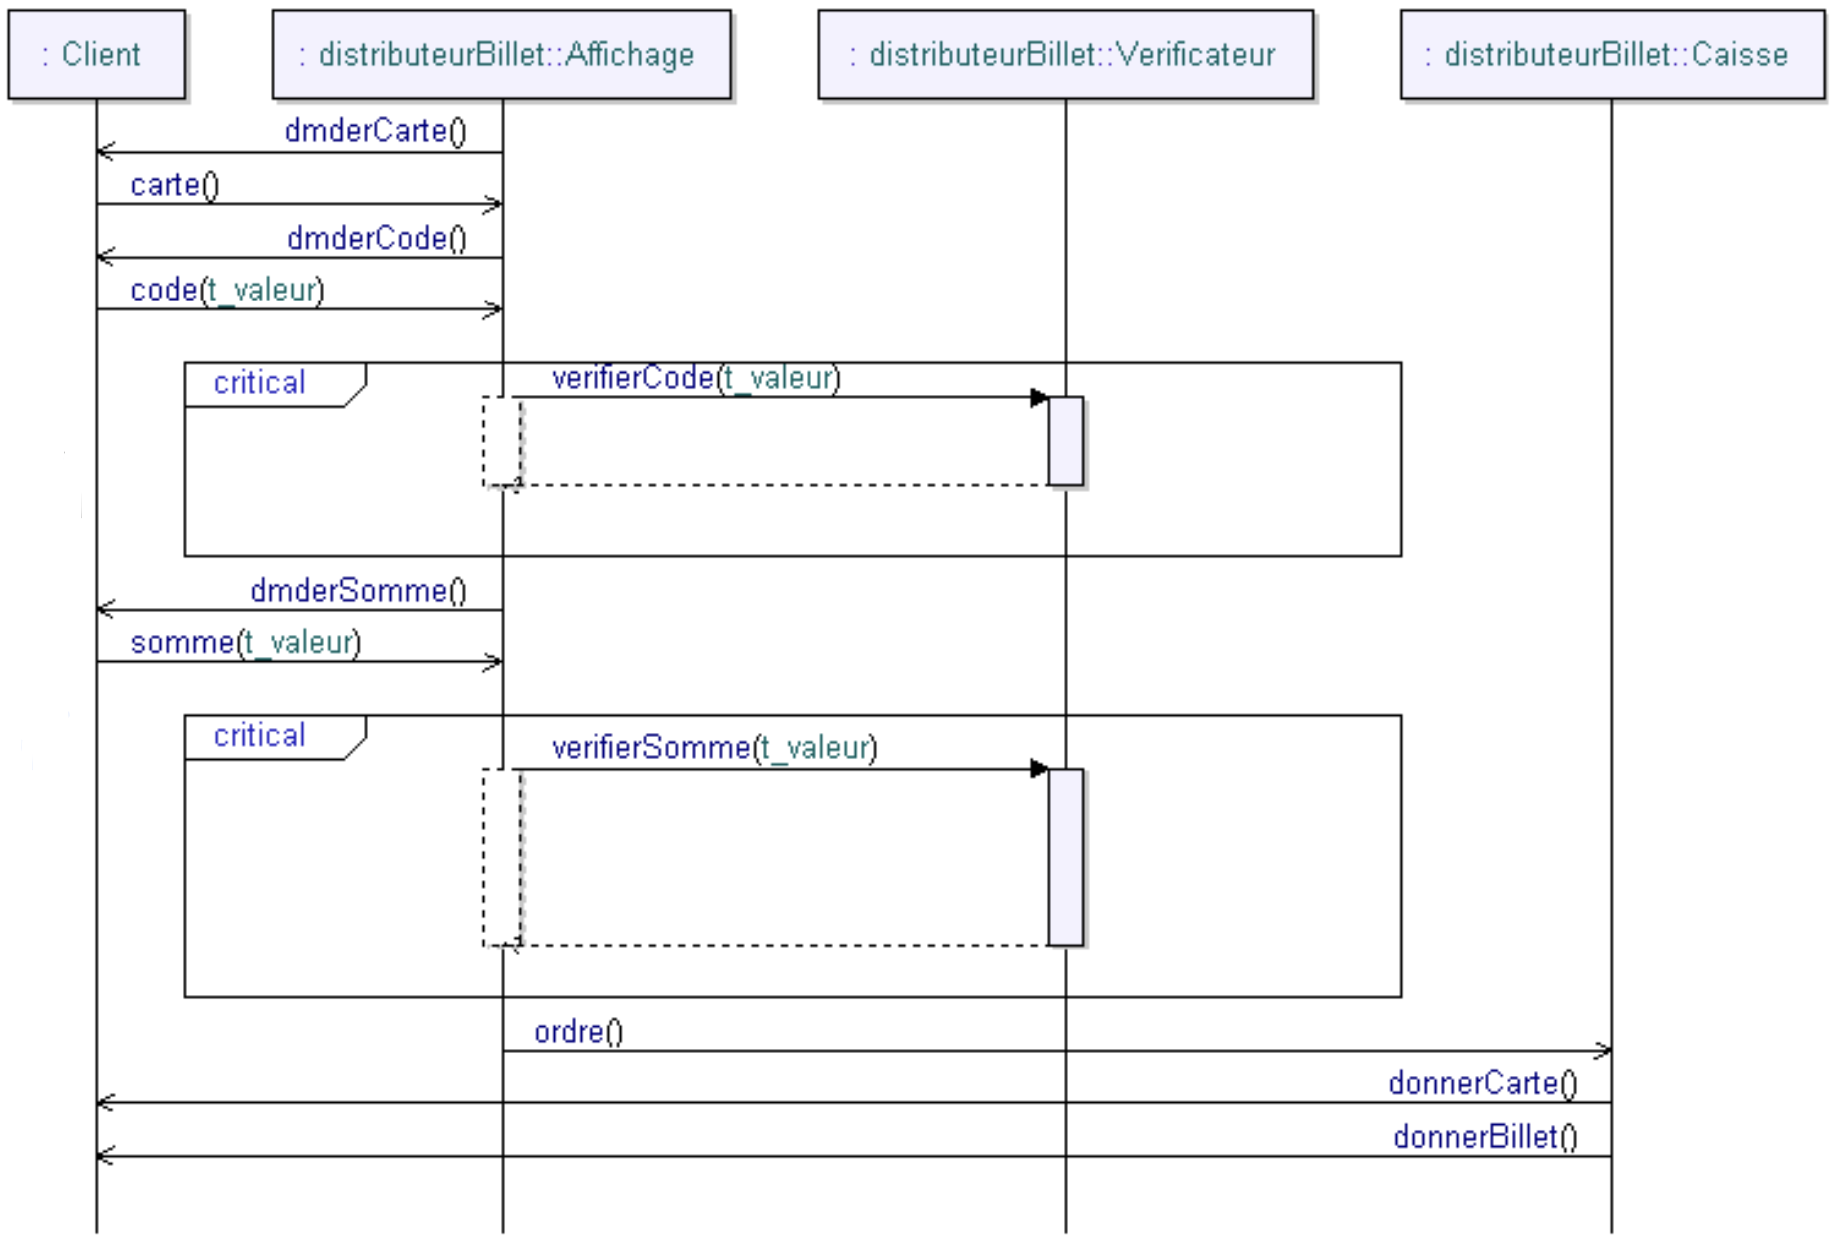
\includegraphics[width=\textwidth]{./Images/Diagrammes/diagram_sequence_fc_critical.png}
\caption{Fragment combiné \og Critical\fg}
\label{fig:diagram_sequence_fc_critical}
\end{subfigure}
\begin{subfigure}{0.45\textwidth}
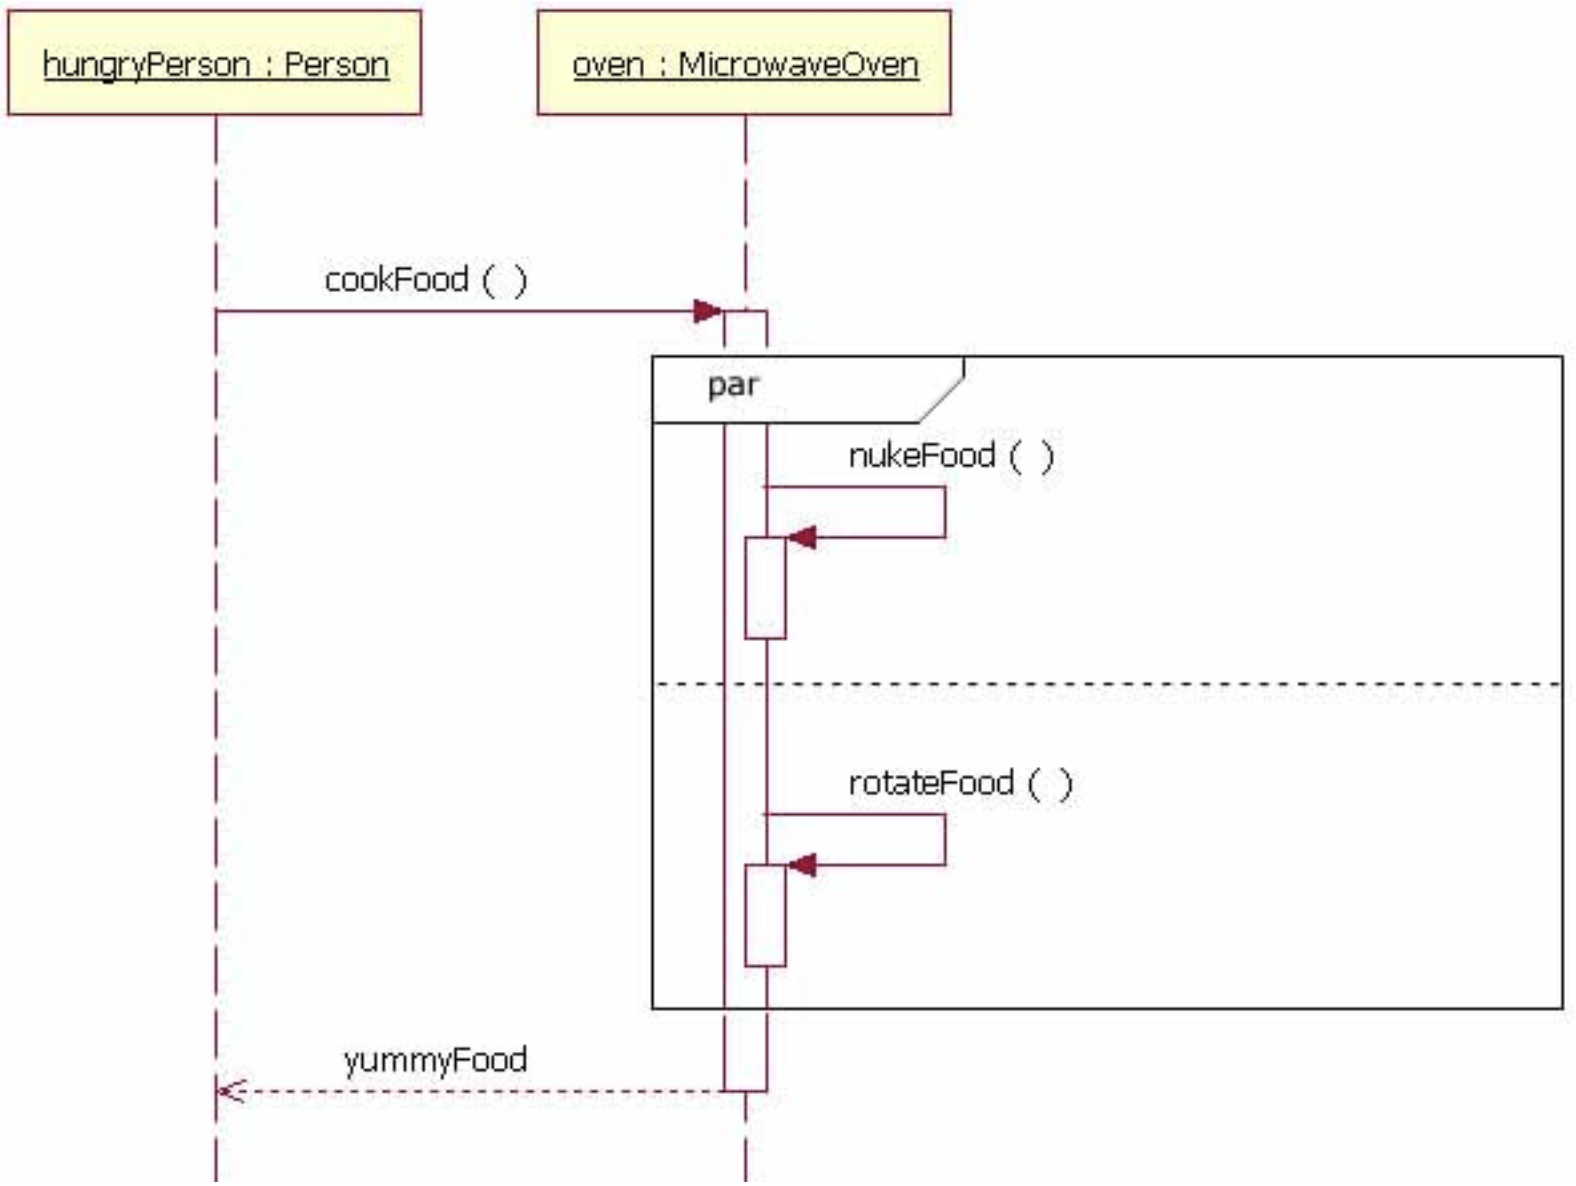
\includegraphics[width=\textwidth]{./Images/Diagrammes/diagram_sequence_fc_par.png}
\caption{Fragment combiné \og Par\fg}
\label{fig:diagram_sequence_fc_par}
\end{subfigure}
\begin{subfigure}{0.45\textwidth}
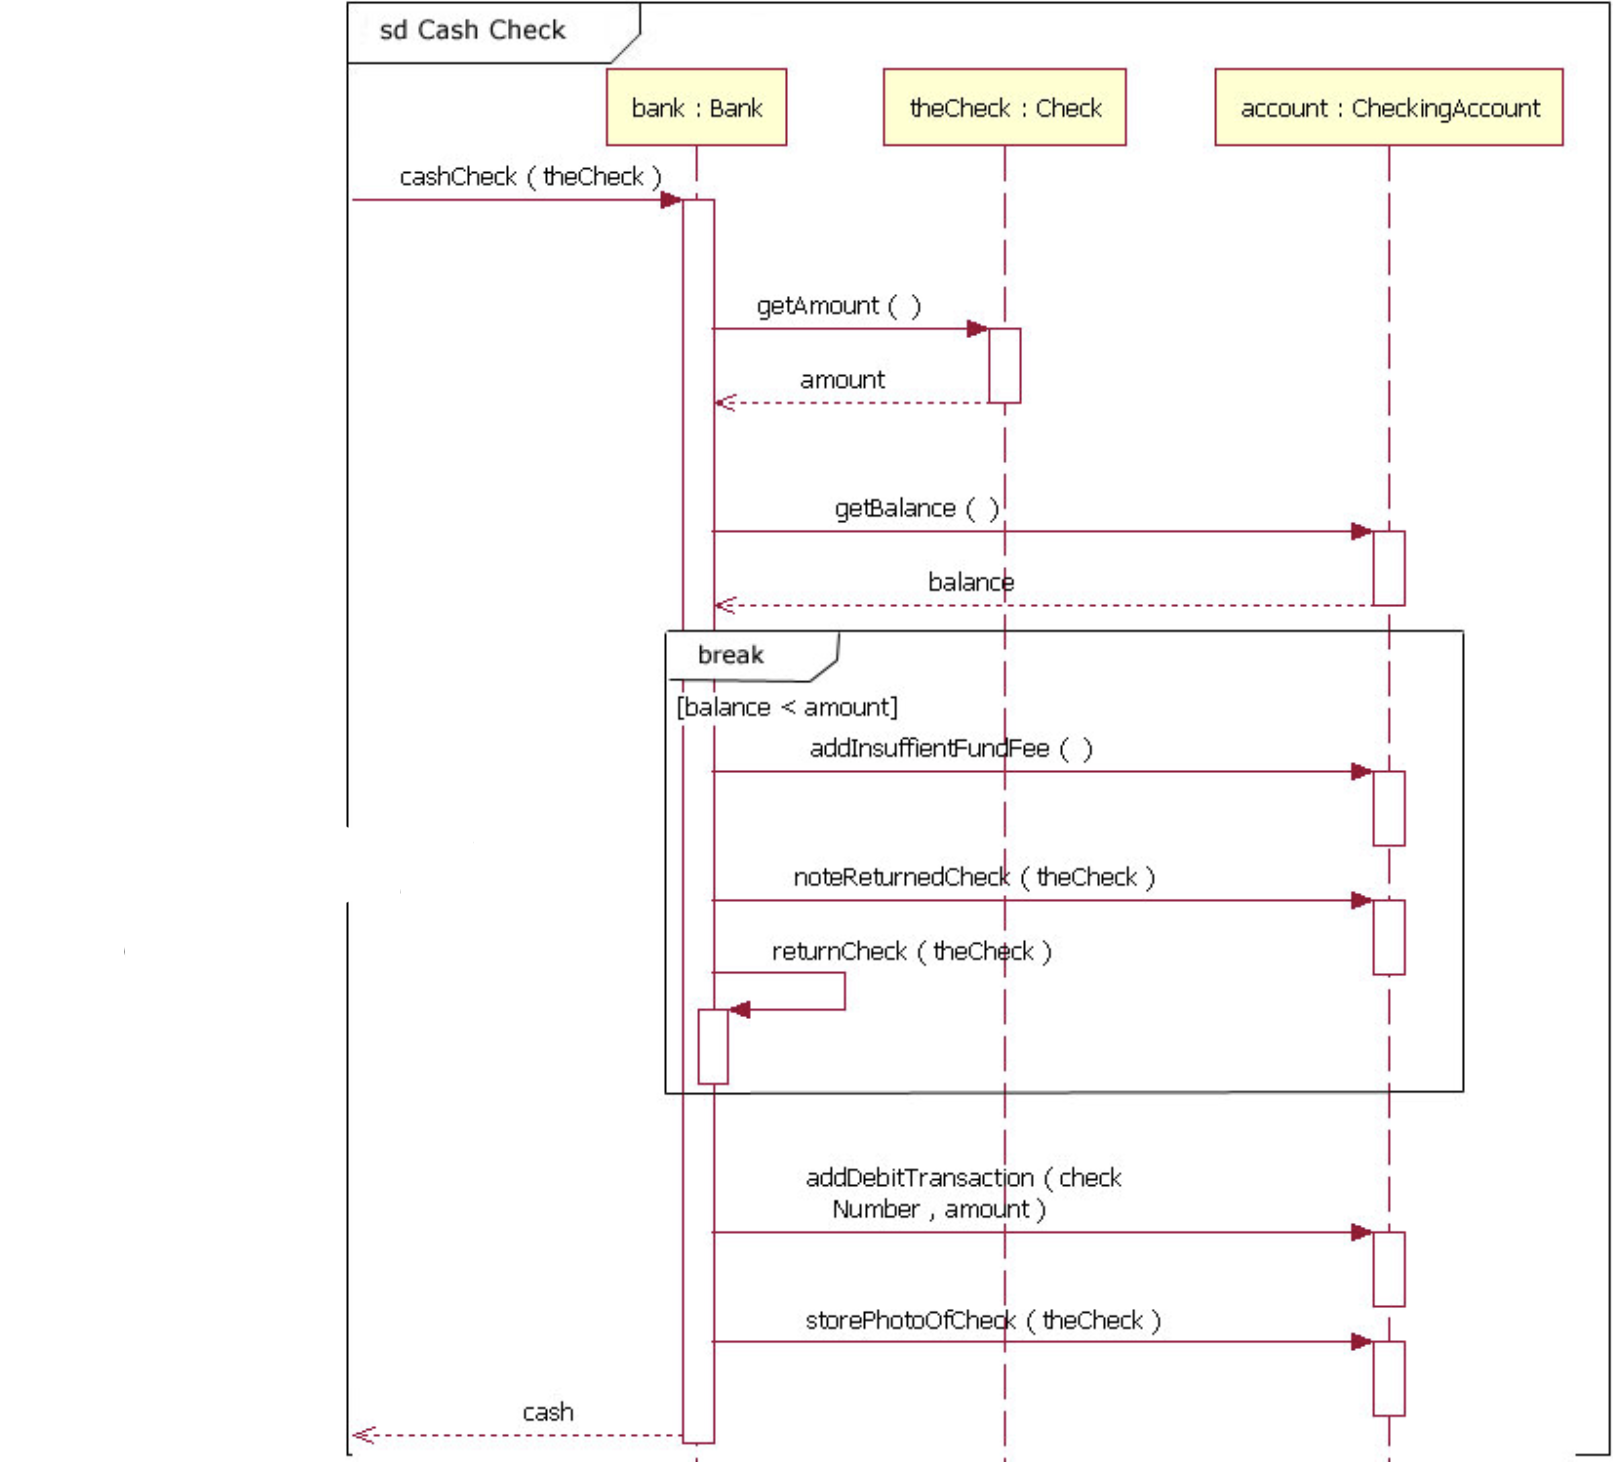
\includegraphics[width=\textwidth]{./Images/Diagrammes/diagram_sequence_fc_break.png}
\caption{Fragment combiné \og Break\fg}
\label{fig:diagram_sequence_fc_break}
\end{subfigure}
\caption{Illustrations des différents types de fragments combinés inclus dans les diagrammes de séquence.}
\end{figure}


